%%%%%%%%%%%%%%%%%%%%%%%%%%%%%%%%%%%%%%%%%
% Programming/Coding Assignment
% LaTeX Template
%
% This template has been downloaded from:
% http://www.latextemplates.com
%
% Original author:
% Ted Pavlic (http://www.tedpavlic.com)
%
% Note:
% The \lipsum[#] commands throughout this template generate dummy text
% to fill the template out. These commands should all be removed when 
% writing assignment content.
%
% This template uses a Cpp script as an example snippet of code, most other
% languages are also usable. Configure them in the "CODE INCLUSION 
% CONFIGURATION" section.
%
%%%%%%%%%%%%%%%%%%%%%%%%%%%%%%%%%%%%%%%%%

%----------------------------------------------------------------------------------------
%	PACKAGES AND OTHER DOCUMENT CONFIGURATIONS
%----------------------------------------------------------------------------------------

\documentclass{article}

\usepackage{fancyhdr} % Required for custom headers
\usepackage{lastpage} % Required to determine the last page for the footer
\usepackage{extramarks} % Required for headers and footers
\usepackage[usenames,dvipsnames]{color} % Required for custom colors
\usepackage{graphicx} % Required to insert images
\usepackage{listings} % Required for insertion of code
\usepackage{courier} % Required for the courier font
\usepackage{lipsum} % Used for inserting dummy 'Lorem ipsum' text into the template
\usepackage{hyperref}
\usepackage{interval}
\hypersetup{
    colorlinks,
    citecolor=black,
    filecolor=black,
    linkcolor=black,
    urlcolor=black
}

% Margins
\topmargin=-0.45in
\evensidemargin=0in
\oddsidemargin=0in
\textwidth=6.5in
\textheight=9.0in
\headsep=0.25in

\linespread{1.1} % Line spacing

% Set up the header and footer
\pagestyle{fancy}
\lhead{\hmwkAuthorName} % Top left header
\rhead{\firstxmark} % Top right header
\lfoot{\lastxmark} % Bottom left footer
\cfoot{} % Bottom center footer
\rfoot{Page\ \thepage\ of\ \protect\pageref{LastPage}} % Bottom right footer
\renewcommand\headrulewidth{0.4pt} % Size of the header rule
\renewcommand\footrulewidth{0.4pt} % Size of the footer rule

\setlength\parindent{0pt} % Removes all indentation from paragraphs

%----------------------------------------------------------------------------------------
%	CODE INCLUSION CONFIGURATION
%----------------------------------------------------------------------------------------

\definecolor{mygreen}{rgb}{0,0.6,0}
\definecolor{mygray}{rgb}{0.5,0.5,0.5}
\definecolor{mymauve}{rgb}{0.58,0,0.82}
\lstloadlanguages{[GNU]C++} % Load Cpp syntax for listings, for a list of other languages supported see: ftp://ftp.tex.ac.uk/tex-archive/macros/latex/contrib/listings/listings.pdf
\lstset{
    backgroundcolor=\color{white},   % choose the background color; you must add \usepackage{color} or \usepackage{xcolor}
    basicstyle=\footnotesize,        % the size of the fonts that are used for the code
    breakatwhitespace=false,         % sets if automatic breaks should only happen at whitespace
    breaklines=true,                 % sets automatic line breaking
    captionpos=b,                    % sets the caption-position to bottom
    commentstyle=\color{mygreen},    % comment style
    deletekeywords={...},            % if you want to delete keywords from the given language
    escapeinside={\%*}{*)},          % if you want to add LaTeX within your code
    extendedchars=true,              % lets you use non-ASCII characters; for 8-bits encodings only, does not work with UTF-8
    frame=single,                    % adds a frame around the code
    keepspaces=true,                 % keeps spaces in text, useful for keeping indentation of code (possibly needs columns=flexible)
    keywordstyle=\color{blue},       % keyword style
    language=[GNU]C++,                 % the language of the code
    otherkeywords={*,...},           % if you want to add more keywords to the set
    numbers=left,                    % where to put the line-numbers; possible values are (none, left, right)
    numbersep=5pt,                   % how far the line-numbers are from the code
    numberstyle=\tiny\color{mygray}, % the style that is used for the line-numbers
    rulecolor=\color{black},         % if not set, the frame-color may be changed on line-breaks within not-black text (e.g. comments (green here))
    showspaces=false,                % show spaces everywhere adding particular underscores; it overrides 'showstringspaces'
    showstringspaces=false,          % underline spaces within strings only
    showtabs=false,                  % show tabs within strings adding particular underscores
    stepnumber=2,                    % the step between two line-numbers. If it's 1, each line will be numbered
    stringstyle=\color{mymauve},     % string literal style
    tabsize=2,                       % sets default tabsize to 2 spaces
    title=\lstname                   % show the filename of files included with \lstinputlisting; also try caption instead of title
}

% Creates a new command to include a Cpp script, the first parameter is the filename of the script (without .cpp), the second parameter is the caption
\newcommand{\cppscript}[2]{
\begin{itemize}
\item[]\lstinputlisting[caption=#2,label=#1]{#1.cpp}
\end{itemize}
}

%----------------------------------------------------------------------------------------
%	DOCUMENT STRUCTURE COMMANDS
%	Skip this unless you know what you're doing
%----------------------------------------------------------------------------------------

% Header and footer for when a page split occurs within a problem environment
\newcommand{\enterProblemHeader}[1]{
\nobreak\extramarks{#1}{#1 continued on next page\ldots}\nobreak
\nobreak\extramarks{#1 (continued)}{#1 continued on next page\ldots}\nobreak
}

% Header and footer for when a page split occurs between problem environments
\newcommand{\exitProblemHeader}[1]{
\nobreak\extramarks{#1 (continued)}{#1 continued on next page\ldots}\nobreak
\nobreak\extramarks{#1}{}\nobreak
}

\setcounter{secnumdepth}{0} % Removes default section numbers
\newcounter{homeworkProblemCounter} % Creates a counter to keep track of the number of problems

\newcommand{\homeworkProblemName}{}
\newenvironment{homeworkProblem}[1][Problem \arabic{homeworkProblemCounter}]{ % Makes a new environment called homeworkProblem which takes 1 argument (custom name) but the default is "Problem #"
\stepcounter{homeworkProblemCounter} % Increase counter for number of problems
\renewcommand{\homeworkProblemName}{#1} % Assign \homeworkProblemName the name of the problem
\section{\homeworkProblemName} % Make a section in the document with the custom problem count
\enterProblemHeader{\homeworkProblemName} % Header and footer within the environment
}{
\exitProblemHeader{\homeworkProblemName} % Header and footer after the environment
}

\newcommand{\problemAnswer}[1]{ % Defines the problem answer command with the content as the only argument
\noindent\framebox[\columnwidth][c]{\begin{minipage}{0.98\columnwidth}#1\end{minipage}} % Makes the box around the problem answer and puts the content inside
}

\newcommand{\homeworkSectionName}{}
\newenvironment{homeworkSection}[1]{ % New environment for sections within homework problems, takes 1 argument - the name of the section
\renewcommand{\homeworkSectionName}{#1} % Assign \homeworkSectionName to the name of the section from the environment argument
\subsection{\homeworkSectionName} % Make a subsection with the custom name of the subsection
\enterProblemHeader{\homeworkProblemName\ [\homeworkSectionName]} % Header and footer within the environment
}{
\enterProblemHeader{\homeworkProblemName} % Header and footer after the environment
}

%----------------------------------------------------------------------------------------
%	NAME AND CLASS SECTION
%----------------------------------------------------------------------------------------

\newcommand{\hmwkTitle}{Competitive Programming Notebook} % Assignment title
\newcommand{\hmwkClass}{ACM/ICPC} % Course/class
\newcommand{\hmwkAuthorName}{Lucas Mattioli, Marlon Mendes, Simi$\tilde{a}$o Carvalho} % Your name

%----------------------------------------------------------------------------------------
%	TITLE PAGE
%----------------------------------------------------------------------------------------

\title{
\vspace{2in}
\textmd{\textbf{\hmwkClass:\ \hmwkTitle}}\\
\vspace{3in}
}

\author{\textbf{\hmwkAuthorName}}
\date{} % Insert date here if you want it to appear below your name

%----------------------------------------------------------------------------------------

\begin{document}

\maketitle

%----------------------------------------------------------------------------------------
%	TABLE OF CONTENTS
%----------------------------------------------------------------------------------------

%\setcounter{tocdepth}{1} % Uncomment this line if you don't want subsections listed in the ToC

\newpage
\tableofcontents
\newpage

%----------------------------------------------------------------------------------------
%	GEOMETRY
%----------------------------------------------------------------------------------------

\section{Points}
\subsection{Comparing floating point values}
Returns true if double values a and b are equal
\cppscript{geometry/src/equals}{equals}


\section{Lines}
\subsection{General equation of a line}
Non-normalized form: ax + by + c = 0
\cppscript{geometry/src/line_general}{General equation of a line}

\subsection{General equation of a line normalized}
\cppscript{geometry/src/line_general_normalized}{General equation of a line}

\subsection{Point on a line}
Is the given point located on the given Line?
\cppscript{geometry/src/line_contains}{Point on line}

\subsection{Equal and parallel lines}
\cppscript{geometry/src/parallel}{}

\subsection{Orthogonal}
\cppscript{geometry/src/orthogonal}{}

\subsection{Intersection}
\cppscript{geometry/src/intersection}{}

\subsection{Angle between lines}
\cppscript{geometry/src/angle_lines}{}

\subsection{Distance to point}
\cppscript{geometry/src/distance_line_point}{}

\subsection{Bissector / Mediatriz}
\cppscript{geometry/src/mediatriz}{}

\subsection{Orientation between point and line}
\cppscript{geometry/src/D}{}

\section{Line segments}

\subsection{Contains point}
\cppscript{geometry/src/segment_contains}{}

\subsection{Closest point}
\cppscript{geometry/src/segment_closest}{}

\subsection{Intersectin with segment}
\cppscript{geometry/src/segment_intersection}{}

\section{Vectors}

\subsection{Angle between vector and X-axis}
Returns an angle in radians in the interval $\interval{-\pi}{+\pi}$. A positive angle means in the COUNTER-clockwise direction. A negative angle is measured in the clockwise direction. Note that the atan2 swaped the parameters.
\cppscript{geometry/src/angle}{angle between X-axis and vector{x, y}}

\subsection{Translation}
\cppscript{geometry/src/translation}{Translate point}

\subsection{Rotation around origin}
\cppscript{geometry/src/rotation}{}

\subsection{Rotation around another point}
\cppscript{geometry/src/rotation_point}{}

\subsection{Rotation around origin 3D}

\begin{center}
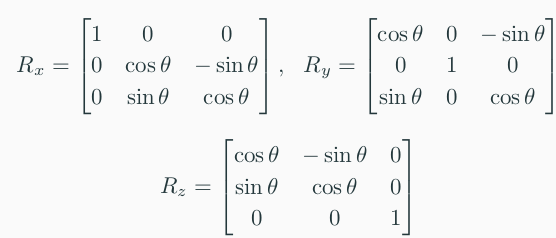
\includegraphics[width = 7in, height = 3.5in]{geometry/images/rotation3d.png}
\end{center}

\subsection{Scale}
\cppscript{geometry/src/scale}{Scale vector by a factor of sx and sy}

\subsection{Normalization}
\cppscript{geometry/src/normalize}{Returns a unit vector with the same direction as the given vector}

\subsection{Dot product}
\[
    <\vec{u}, \vec{v}> = \vec{u} \cdot \vec{v} = u_xv_x + u_yv_y = |\vec{u}||\vec{v}|\cos \theta
\]

\cppscript{geometry/src/dot}{}

\subsection{Angle between vectors}
\cppscript{geometry/src/angle_vectors}{}

\subsection{Cross product}

$
            u\times v = \begin{vmatrix}
                \vec{i} & \vec{j} & \vec{k} \\
                u_x & u_y & u_z \\
                v_x & v_y & v_z \\
            \end{vmatrix}
$
\begin{itemize}
\item $|\vec{u}\times \vec{v}| = |\vec{u}||\vec{v}|\sin \theta$
\item where $\vec{i}, \vec{j}, \vec{k}$ are unity vectors on the same direction and orientation as $x, y, z$, respectively
\item the result vector $\vec{w}$ is orthogonal to both $\vec{u}$ and $\vec{v}$
\item it is the area of the parallelogram formed by $\vec{u}$ and $\vec{v}$
\end{itemize}

\cppscript{geometry/src/cross}{}

\section{Circles}

\subsection{Definition}
\cppscript{geometry/src/circle_definition}{}

\subsection{Perimeter, Area}
\cppscript{geometry/src/circle_perimeter}{}

\subsection{From 2 points}
\cppscript{geometry/src/circle_from_2_points}{}

\subsection{From 3 points}
\cppscript{geometry/src/circle_from_3_points}{}

\subsection{Intersection between 2 circles}
\cppscript{geometry/src/circle_intersection}{}

\subsection{Intersection between circle and line}
\cppscript{geometry/src/inter_line_circle}{}

\subsection{Intersection between circle and point}
\cppscript{geometry/src/circle_point}{}

\section{Triangles}

\subsection{Perimeter}
\cppscript{geometry/src/triangle/perimeter}{}

\subsection{Area}
\cppscript{geometry/src/triangle/area}{}
\cppscript{geometry/src/triangle/area2}{}
\cppscript{geometry/src/triangle/area3}{}


\subsection{Side classification}
\subsubsection{By sides}
\cppscript{geometry/src/triangle/classification_by_sides}{}
\subsubsection{By angles}
\cppscript{geometry/src/triangle/classification_by_angles}{}

\subsection{Important points}
\subsubsection{Barycenter}
\cppscript{geometry/src/triangle/barycenter}{}
\subsubsection{Incenter}
\cppscript{geometry/src/triangle/incenter}{}
\subsubsection{Orthocenter}
\cppscript{geometry/src/triangle/orthocenter}{}
\subsubsection{Circumcircle}
\cppscript{geometry/src/triangle/circumcircle}{}

\section{Quadrilaterals}

\subsection{Area}
\subsubsection{Trapezium}
\cppscript{geometry/src/quadrilateral/trapezium}{}
\subsubsection{Quadrilateral}
\cppscript{geometry/src/triangle/area}{}

\subsection{Rectangles}
\subsubsection{From 2 points}
\cppscript{geometry/src/quadrilateral/rect}{}
\subsubsection{Intersection between rectangles}
\cppscript{geometry/src/quadrilateral/intersection}{}

\clearpage


%----------------------------------------------------------------------------------------

\end{document}
